\section{Methodology}

The identification of use cases for the \textit{TenSyGrid} Toolbox follows a user-centred design approach, placing the network operator or converter designer, for instance, as the primary actor. Use cases were derived from three complementary sources:

\begin{enumerate}
  \item \textbf{Project objectives.} The TenSyGrid proposal defines the toolbox as a stability assessment platform for converter-dominated power grids. The core workflow --- load a grid model, run a small-signal stability analysis, and interpret the results --- directly informs the first set of use cases.
  \item \textbf{Feedback with GUI prototype and group members.} An initial web-based Stability Monitor has been developed, implementing five core interaction flows: simulation execution (UC-01), system status monitoring and eigenvalue analysis (UC-02), critical mode inspection (UC-03), bus voltage evaluation (UC-04), and $N-1$ contingency assessment (UC-05). These flows were formalised as the implemented use cases. From meetings with group colleagues, the definition of the proposed use cases has been done.\\
  CAMBIAR\\ 
  \item \textbf{Industry needs analysis.} From interviews with different agents in the industry, additional use cases (UC-06 to UC-14) have been drafted to explore workflows that go beyond single-snapshot analysis, including scenario comparison, trend monitoring, and actionable recommendations.
\end{enumerate}

Each use case is described following a structured template that includes \textbf{identifier} and \textbf{name}, \textbf{actor}, \textbf{objective}, \textbf{preconditions}, \textbf{theoretical basis}, \textbf{possible bottlenecks}, \textbf{main flow}, \textbf{GUI interaction}, and \textbf{expected result}.

It is important to note that all use cases are designed to follow Shneiderman's approach \cite{shneiderman1996eyes} and support a progressive analysis workflow. In practical terms, the user can:

\begin{enumerate}
  \item Obtain an overview of the system status.
  \item Zoom into critical modes and their physical origin.
  \item Filter and sort the eigenvalue spectrum to focus on the most relevant dynamics.
  \item Derive actionable recommendations for control design or contingency mitigation.
\end{enumerate}

This structure ensures that the toolbox supports both rapid operational screening and deeper technical diagnosis when required broadening the information about the grid getting into each of the proposed use cases.

\section{Tool scheme and structure}

\subsection{Initial tool scheme and architectural evolution}

\paragraph{Initial Conceptual Scheme (Figure~\ref{fig:tool_scheme}).}
At the outset of the TenSyGrid project, the preliminary architectural roadmap considered MATLAB as a key foundation of the development platform. This initial strategy was primarily motivated by the pre-existing research legacy within the consortium, specifically the Multilinear Time-Invariant (MTI) Toolbox developed in earlier and concurrent project stages~\cite{Kaufmann2025TenSyGridD11,Wong2025TenSyGridD21}, alongside the STAMP simulation framework. In this early phase, before key design decisions regarding runtime dependencies were finalized, the toolbox was conceived as a hybrid, multi-branch framework connecting open-source components with existing MATLAB prototypes through dedicated runtime adapters.

This initial conceptual architecture is illustrated in Figure~\ref{fig:tool_scheme}. As originally planned, the platform established two parallel simulation branches:
\begin{enumerate}[before=\leavevmode, leftmargin=*]
  \item \textbf{VeraGrid Platform (Python):} Designed as an open-source modeling environment incorporating modular calculation engines for power flow ($\text{VG}_\text{PF}$), dynamic root-mean-square transient simulations ($\text{VG}_\text{RMS}$), small-signal stability analysis ($\text{VG}_\text{SSig}$), and a dedicated multilinear/tensor integration layer ($\text{VG}_\text{MTI}$).
  \item \textbf{STAMP and MTI Framework (MATLAB):} Encapsulating the original MTI tensor formulation and STAMP power-flow ($\text{S}_\text{PF}$), electromagnetic transient ($\text{S}_\text{EMT}$), and small-signal ($\text{S}_\text{SSig}$) routines, intended to interact with Python via bi-directional process adapters.
  \item \textbf{Interoperability Layer (IPSA):} Envisioned to ingest network topologies and dynamic controller parameters from external industry-standard tools (PSCAD, DIgSILENT PowerFactory, PSS/E, MATLAB/Simulink).
\end{enumerate}

\begin{figure}[H]
  \centering
  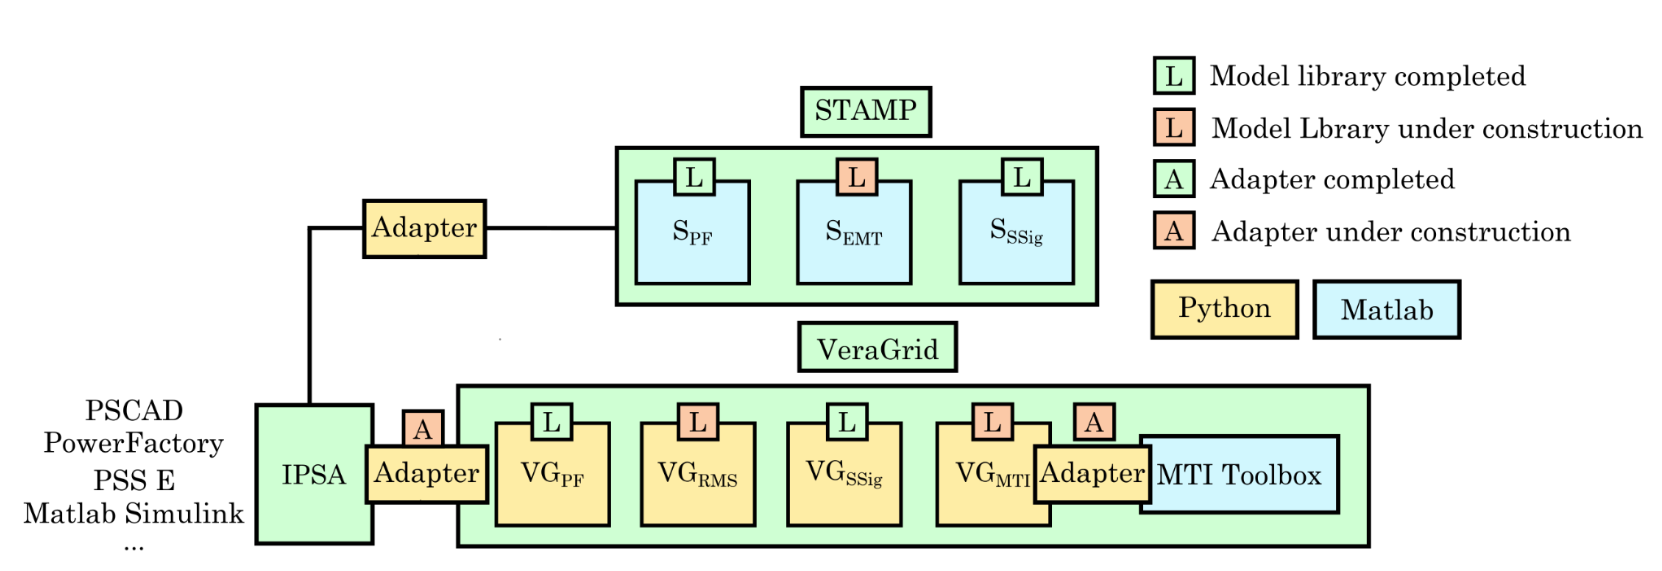
\includegraphics[width=0.85\textwidth]{pictures/esquema.png}
  \caption[Initial TenSyGrid modular scheme and hybrid integration concept.]{Initial conceptual scheme of the TenSyGrid toolbox, conceived during early project stages prior to resolving the MATLAB software dependency. In this preliminary design, external models fed into VeraGrid (Python) while relying on runtime adapters to bridge into MATLAB-based MTI and STAMP simulation packages.}
  \label{fig:tool_scheme}
\end{figure}

\paragraph{The MATLAB Decision and Strategic Architectural Pivot.}
Although this initial hybrid layout enabled early prototyping by recycling legacy MATLAB scripts, in-depth evaluation revealed that maintaining a dependency on MATLAB was incompatible with the operational, technical, and regulatory requirements of a production-grade toolbox for Transmission System Operators (TSOs):
\begin{itemize}[before=\leavevmode, leftmargin=*]
  \item \textbf{Licensing and Open-Source Distribution:} MATLAB is commercial proprietary software subject to strict per-seat or concurrent network licensing. Requiring proprietary licenses creates a severe barrier for widespread dissemination among TSOs, academic researchers, and industrial stakeholders. A core requirement of the European CETPartnership initiative is fostering fully accessible, transparent, and reproducible tooling, necessitating a zero-cost, open-source distribution model.
  \item \textbf{Supercomputing and Cloud Scalability:} Assessing small-signal stability in modern converter-dominated grids demands computationally intensive batch runs, including massive $N-1$ contingency evaluations, broad parameter sweeps, and Monte Carlo-based renewable scenario assessments. In High-Performance Computing (HPC) clusters and cloud environments (e.g., managed via SLURM or container orchestration platforms), MATLAB license-token checkouts severely constrain parallel scaling across hundreds of worker nodes. In contrast, Python runs natively in headless Linux containers (e.g., Docker, Apptainer/Singularity) and leverages distributed computing paradigms without licensing bottlenecks.
  \item \textbf{Adapter Complexity and Runtime Fragility:} Bridging Python and MATLAB at runtime required IPC adapters, cross-language data serialization, and dual-runtime environments. This increased software maintenance overhead, introduced memory transfer latencies, and complicated installation on control-room workstations.
  \item \textbf{Unified Scientific and Web Ecosystem:} The modern Python scientific stack (NumPy, SciPy, sparse matrix solvers, and compiled acceleration libraries) provides numerical performance on par with or exceeding MATLAB, while modern asynchronous frameworks (such as FastAPI) enable seamless coupling with web-based operational monitoring interfaces.
\end{itemize}

Consequently, the consortium formally decided to eliminate the MATLAB dependency entirely and pivot to a 100\% native Python architecture. The tensor formulation and multilinear algorithms of the MTI Toolbox were re-engineered directly into Python within the dedicated \texttt{TensyGridEngine}, built seamlessly on top of \texttt{VeraGridEngine}.


\subsection{Integrated tool architecture and operational workflow}

Following the decision to transition away from MATLAB, the initial hybrid concept of Figure~\ref{fig:tool_scheme} evolved into the streamlined, end-to-end computational and visualization pipeline shown in Figure~\ref{fig:tool_pipeline}. This final architecture eliminates all external runtime bridges and provides a clean, four-stage data flow from external model ingestion to the operator interface:

\begin{figure}[H]
  \centering
  \definecolor{schemepass}{RGB}{203, 245, 216}   % #CBF5D8 (mint green - IPSA)
  \definecolor{schemepython}{RGB}{254, 232, 157} % #FEE89D (soft yellow - Python / VeraGrid)
  \definecolor{schemematlab}{RGB}{189, 227, 251} % #BDE3FB (soft blue - Web / MATLAB)
  \begin{tikzpicture}[
      font=\small,
      >=Latex,
      node distance=7.5mm,
      stagebox/.style={
          rectangle,
          draw=black,
          line width=0.9pt,
          inner sep=5.5pt,
          text width=14.0cm,
          align=left
        },
      flowarrow/.style={
          ->, line width=1.1pt, draw=black
        },
      arrowlabel/.style={
          font=\scriptsize, text=black, fill=white, draw=black!50, line width=0.4pt, inner sep=2pt, rounded corners=1pt
        }
    ]

    % Stage 1: Ingestion (IPSA Green)
    \node[stagebox, fill=schemepass] (stage1) {
      \textbf{\normalsize 1. External Model Ingestion} \hfill \textsf{\footnotesize [IPSA Adapter]} \\[2pt]
      \textbullet~Ingests grid topology, equipment parameters, and dynamic controller models from external commercial tools (PSCAD, DIgSILENT PowerFactory, PSS/E, MATLAB/Simulink). \\
      \textbullet~Standardizes network definitions and dynamic parameter structures for downstream simulation.
    };

    % Stage 2: VeraGrid Engine (Python Yellow)
    \node[stagebox, fill=schemepython, below=of stage1] (stage2) {
      \textbf{\normalsize 2. Grid Modeling \& Operating Point Solution} \hfill \textsf{\footnotesize [VeraGridEngine]} \\[2pt]
      \textbullet~Instantiates internal \texttt{MultiCircuit} model (buses, branches, generators, converters, loads, shunts). \\
      \textbullet~Attaches dynamic phasor RMS templates and performs algebraic descriptor conversion (\texttt{to\_implicit}). \\
      \textbullet~Solves AC/DC Power Flow (\texttt{vge.power\_flow}) to establish the pre-disturbance equilibrium state $\mathbf{x}_0$.
    };

    % Stage 3: TenSyGrid Engine (Python Yellow)
    \node[stagebox, fill=schemepython, below=of stage2] (stage3) {
      \textbf{\normalsize 3. Multilinear Stability \& Contingency Engine} \hfill \textsf{\footnotesize [TensyGridEngine]} \\[2pt]
      \textbullet~\textbf{Descriptor Assembly:} Builds multilinear system $\mathbf{E}\dot{\mathbf{x}}=\mathbf{A}\mathbf{x}$ using \texttt{RmsProblemMultilinear}. \\
      \textbullet~\textbf{Modal Analysis:} Solves $\lambda_k\mathbf{E}\mathbf{v}_k=\mathbf{A}\mathbf{v}_k$ to extract damping ratios $\zeta_k$, frequencies $f_k$, and participation factors $p_{ki}$ (\texttt{small\_signal\_analysis\_main.py}). \\
      \textbullet~\textbf{$N-1$ Contingency Screening:} Iteratively disconnects transmission elements to evaluate post-fault security margins (\texttt{run\_contingency.py}), caching results into \texttt{.tensygrid} files.
    };

    % Stage 4: GUI / Stability Monitor (Web / Soft Blue)
    \node[stagebox, fill=schemematlab, below=of stage3] (stage4) {
      \textbf{\normalsize 4. Operational \& Diagnostic Interface} \hfill \textsf{\footnotesize [FastAPI Backend \& Web GUI]} \\[2pt]
      \textbullet~\textbf{REST Backend:} Asynchronous service (\texttt{dashboard.py}) managing runs and precomputed caches. \\
      \textbullet~\textbf{Stability Monitor (\texttt{index.html}):} Executive status badges (green/yellow/red), complex-plane eigenvalue plot ($\sigma \pm j\omega$), critical mode participation ranking, $N-1$ contingency tables, and voltage profiles.
    };

    % Connections with clear vertical space and visible arrows
    \draw[flowarrow] (stage1.south) -- node[arrowlabel, midway] {Standardized grid definitions \& dynamic parameters} (stage2.north);
    \draw[flowarrow] (stage2.south) -- node[arrowlabel, midway] {Operating point $\mathbf{x}_0$ \& implicit phasor equations} (stage3.north);
    \draw[flowarrow] (stage3.south) -- node[arrowlabel, midway] {Eigenvalues, damping ratios, participation factors \& contingency outcomes} (stage4.north);

  \end{tikzpicture}
  \caption[Final integrated tool architecture and operational workflow.]{Final integrated architecture and computational workflow of the TenSyGrid toolbox, adopted following the architectural decision to transition from the initial MATLAB-dependent hybrid scheme to a fully native open-source Python stack. The four-stage pipeline spans external model ingestion, VeraGrid modeling, native TenSyGrid multilinear stability analysis, and the operator web interface.}
  \label{fig:tool_pipeline}
\end{figure}

The modular decoupling illustrated in Figure~\ref{fig:tool_pipeline} ensures clear separation of concerns across the pipeline:
\begin{enumerate}[before=\leavevmode, leftmargin=*]
  \item \textbf{Ingestion and standardisation:} Downstream computational modules remain completely agnostic to the proprietary origins of the network models, relying exclusively on standard internal interfaces.
  \item \textbf{High-performance core computing:} Heavy numerical operations (power flow, descriptor matrix assembly, generalized eigenvalue solves, and batch contingency runs) run natively in optimized C++/Python libraries on dedicated servers or HPC compute nodes.
  \item \textbf{Zero-footprint operator access:} Transmission operators access results through an intuitive, lightweight web browser interface without needing local numerical software or specialized compiler toolchains installed on control-room workstations.
\end{enumerate}



\section{Operator interviews}
To ground the use-case catalogue in real operational practice, three semi-structured interviews were conducted with transmission-system stakeholders; the key findings that shaped the use cases are summarised below.

\paragraph{eRoots; former TSO planner and control-room analyst at XM, Colombia.} They described the operational workflow at XM: economic dispatch coordinated in 8-hour shifts, system validation every 15--30 minutes, and \mbox{$N-1$} contingency screening complemented by short-circuit and RMS dynamic simulations for critical cases. On the planning side, detailed modelling of low-voltage networks and IBRs (including protection systems) overloaded the state-space representation, making small-signal studies (SSTI, SSSI, SSOS) take 3--4 hours. Key operational metrics were the frequency nadir, ROCOF, and the settling time $T_{1090}$; in planning, eigenvalue position, damping, SCR variation, and participation factors were used to avoid out-of-band interactions. Regarding the GUI prototype, he recommended: (i) removing traffic-light indicators while keeping colour coding in the complex plane; (ii) providing explicit error debugging when a simulation fails; (iii) linking eigenvalues and participation factors to specific devices and state variables ($\omega$) to distinguish local from inter-area oscillations; (iv) adding visualisation of operational bands (P-V curves); and (v) supporting sequential contingencies (chains of events, $N$-$2$) and multiple simultaneous contingency selection (e.g.\ via YAML configuration).

\paragraph{Project Leader of HDVC at Siemens Energy.} They outlined three families of studies performed in the HVDC context: (i) \emph{dynamic performance} of an HVDC link under grid events, run in EMT with hundreds of PSCAD cases over 1-2 days; (ii) \emph{RMS} whole-country contingency screening ($N$-$1$) on AC networks of the order of 500\,km radius (e.g.\ UK GB network), taking a few hours; and (iii) \emph{screening studies} to identify synchronous generators that may interact problematically with the HVDC, run as load-flow and short-circuit analyses in minutes. He noted that small-signal studies are currently performed through impedance scanning (SS-SFI), with the frequency response obtained from PSCAD; clients are beginning to request state-space models (grey-box, per subsystem) for which a Laplace transfer function may be delivered instead, keeping the full model confidential for security reasons. He also highlighted harmonic-stability assessment based on gain/phase margins rather than eigenvalues, and the need to study voltage collapse in weak grids, which linear mode analysis does not capture. Automation of simulation campaigns and of result post-processing was identified as a key unmet need.

\paragraph{European mainland TSO.} They described the planning and operational processes at Elia: long-term grid development (TYDP, every two years), short-term planning, and operational processes from week-ahead down to intraday and real-time (SCADA/EMS with state estimation). Models are exchanged in CGMES; PowerFactory, PSCAD, and SCADA are the three main software tools. Dynamic security assessment (DSA) involves thousands of contingency cases; computation time limits model detail, and the trade-off is managed by increasing the number of cores. Day-ahead studies use RMS (PowerFactory); close to real time, about 100 cases are run with reduced detail. Outage management is not automatic and there is interest in AI tools to judge criticality. Regarding HVDC, he noted that all operators previously provided Thevenin equivalents and now need to provide reduced models; any tool deployed must integrate with the existing commercial software stack. On model exchange, he questioned how complete CGMES is for dynamic data and mentioned German colleagues working on software-independent EMT models, pointing to VeraGrid as a relevant platform.

These interviews directly motivated the proposed use cases: scenario comparison and trend analysis (UC-06, UC-08) address the need to track stability across the planning horizon and multiple contingencies; critical-element ranking (UC-09) and damping-controller placement (UC-10) respond to the request to link modes to specific devices; centre-manifold analysis (UC-13) and basin-of-attraction estimation (UC-14) target the weak-grid and large-disturbance questions. The request for clear error debugging, device-level attribution, and operational bands feeds directly into the GUI interaction design of the implemented use cases (UC-01 to UC-05).
